\section{Implementation}
\label{sec:implementation}

%Application of Singular Value Decomposition to FEM results compression

The objective of the compression algorithm is to reduce amount of data representing FEM results and also the ability to reconstruct original data from its smaller representation. This saves storage capacity and also accelerates data transfer between computers as the analysis itself and the post-processing of results is usually done on different work stations.

Compression method can be lossy or lossless based on quality of data reconstructed of its compressed representation. Lossless methods are able to fully recreate original data. Lossy methods on the other hand produce only approximations of original data. 

SVD is used as part of the compression algorithm. SVD method applied to arbitrary matrix produces decomposition that consist of corresponding singular values and singular vectors. This process is fully reversible (with the assumption that the numerical errors are negligible). The original matrix can be reconstructed by the multiplication of decomposed parts. However, the compression algorithm is based on modification of decomposition to create \textbf{low-rank approximation matrix}. The reconstructed matrix slightly differs from the original matrix and algorithm therefore does \textbf{lossy} compression.

% jak ziskam matici na kterou aplikuji SVD? popsat z ceho se skladaji fem data a jak se naskladaji do matice

SVD decomposition is applied on matrices. The first thing to do is therefore to assemble an input matrix. Results from the Finite element method are discrete values calculated in nodes or integration points. There are usually multiple fields in result data (e.g. Displacements, Stress, Strain etc.) and each field can have multiple components (e.g. Displacements can have $X$, $Y$ and $Z$ component). As non-linear analyses usually lead to multiple computation steps there are multiple sets of data per each field component. All data corresponding to a single field component forms the input matrix to the compression algorithm. Let's call it matrix $\mtrx{A}$. Each row of matrix $\mtrx{A}$ corresponds to single time step and each column correspond to single node or integration point.

Once the matrix $\mtrx{A}$ is build for a field component the compression algorithm can be applied on it. It is purely algebraic procedure, no information about geometry of the mesh is needed.

The compression algorithm is based on low-rank approximation matrix created from SVD decomposition. The main idea that led to this implementation is the following observation. Results for time steps are not independent. They have some relation between them. List of singular values produced by the SVD method reveals the dependency between the singular vectors that form the orthogonal base of the matrix $\mtrx{A}$. \todo{Better explanation needed}

Only single field component is considered to fill the input matrix $\mtrx{A}$. Results for different data components, even for the same field, can be independent from each other. There can also be order-of-magnitude difference between the components and the compression algorithm could potentially clear the important information in the weaker component. Another reason against merging of components is computational complexity. The smaller the matrix $\mtrx{A}$ is, the faster the decomposition algorithm performs.

\subsection{Low-rank approximation matrix}

\todo[inline]{Pokracovat vysvetlenim aproximace pomoci matice s nizsi hodnosti. Inspirovat se clankem \cite{SairaBanu2015}, pridat rovnice a diagram}

From the properties of SVD method presented in section \ref{sec:math} it follows the fact that a matrix can be represented in the form of its SVD components as a sum of rank 1 matrices in the form

$$\mtrx{A}=\mtrx{U_{1}}S_{1}\mtrx{V_{1}^{T}}+\mtrx{U_{2}}S_{2}\mtrx{V_{2}^{T}}+ ... +\mtrx{U_{n}}S_{n}\mtrx{V_{n}^{T}}$$

where $S_{i}$ is $i$-th singular value, $U_{i}$, $V_{i}$ are corresponding singular vectors, and $n$ is the rank of the matrix $\mtrx{A}$. Considering the fact that singular values are ordered $S_{1}>S_{2}>S_{3}> ... >S_{n}$ the above formula implies that the first term would have the highest contribution and last term would have the lowest contribution to the matrix~$\mtrx{A}$. Therefore if we take only first $r$ members of the above summation we get approximation of the matrix $\mtrx{A}$

$$\mtrx{A'}=\mtrx{U_{1}}S_{1}\mtrx{V_{1}^{T}}+\mtrx{U_{2}}S_{2}\mtrx{V_{2}^{T}}+ ... +\mtrx{U_{r}}S_{r}\mtrx{V_{r}^{T}}$$

The quality of approximation depends on the magnitude of the singular values omitted from the approximation formula, namely $S_{r+1} ...  S_{n}$. The compression algorithm is based on assumption that the first singular value is order-of-magnitude higher than singular values at the end of the decomposition sequence. In special cases, when $r=n$, or $S_{i}=0$ for all $i \geq r$ the omitted singular values do not contribute to the sum and the compression is therefore loss-less. In other cases approximation error has to be calculated and taken into account to avoid loss of important details in data.

The main goal of the compression algorithm is to find a compromise between low approximation error and high compression ratio $CR$ which is calculated using the formula

$$CR=\frac{r(m+n+1)}{m n}$$

where $m$ and $n$ are dimensions of matrix $\mtrx{A^{m \times n}}$. Explanation of the compression ratio formula is best done using Figure~\ref{fig:lowrank_svd}. Light color represents the part of matrix decomposition that is to be stored in the output file as a low-rank approximation of the input.

\begin{figure}[ht]
\centering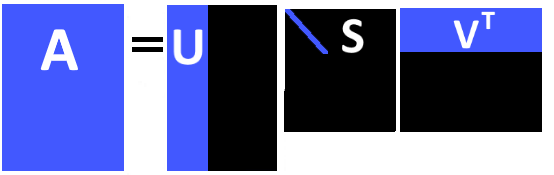
\includegraphics[width=0.7\textwidth]{figures/low_rank_decomposition_diagram}
\caption{Decomposition of input matrix $\mtrx{A}$ into diagonal matrix of singular values $\mtrx{\Sigma}$ and matrices of left and right singular vectors. Light color illustrates low-rank approximation.}
\label{fig:lowrank_svd}
\end{figure}

Let us assume that the matrix is not empty and has full-rank. Then from the formula above follows that if $r$ equals to the rank of matrix $\mtrx{A}$ the compression ratio is always higher than one. In other words the memory consumption of stored decomposition is bigger than the size of the original matrix. To compression algorithm be applicable the parameter $r$ must conform to the condition

$$r<\frac{m n}{m+n+1}$$

Considering the usual shape of matrix containing FEM results this inequality is easily satisfiable even for the $r$ being close to the rank of the original matrix as in the typical case the number of nodes or integration-points is much higher than the number of analysis steps and therefore $m<<n$.

\todo[inline]{jak se pocita chyba; jak se da ridit maximalni chyba}

\subsection{Algorithm description}

\todo[inline]{algorithm steps ... popsat to, co se deje ve funkci Compress v SvdCompressionService, nepopisovat samotnou SVD, to by melo byt popsanot v sekci Mathematical background}

\subsection{Optimization}

\todo[inline]{At first: algorithm complexity (kniha od JK os SVD - je tam slozitost algoritmu); table with execution times...}

\todo{pridat odvozeni}
Complexity: $mn^2$ where $m \leq n$ % http://mathoverflow.net/questions/161252/what-is-the-time-complexity-of-truncated-svd

\todo[inline]{Then main features for optimization: key time steps (time step span compression), Randomized SVD, Parallelization, Sparse matrix of details, prenasobeni U matice singularnimi cisly, trochu usetrim pamet...}
